\documentclass[12pt,letterpaper,reqno]{amsart}
\usepackage{enumerate}
\usepackage[shortlabels]{enumitem}
\usepackage{graphicx}
\usepackage{amssymb}
\usepackage[normalem]{ulem}
\usepackage{titlesec,bbm, hyperref}
\usepackage{spverbatim} 
\usepackage{esvect}
\usepackage{geometry}
\usepackage{caption}
\usepackage{subcaption}
\geometry{letterpaper, portrait, margin=0.5in}

\newcommand{\R}{\mathbb R}

\begin{document}

\thispagestyle{empty}
\centerline{\Large Math 675 Homework 2}
\centerline{Sumanth Ravipati}
\centerline{9/4/2018}
\vspace{.25in}

\begin{enumerate}[1.]
\item (2 points) Prove the Cauchy-Schwartz inequality, following Problem 2 on Page 45.
\begin{flushleft}
$$ \frac{1}{2}\sum\limits_{i=1}^n\sum\limits_{j=1}^n(a_i b_j - b_i a_j)^2 = \frac{1}{2}(\sum\limits_{i=1}^n\sum\limits_{j=1}^n(a_i^2 b_j^2 + b_i^2 a_j^2 - 2 \cdot a_i b_i a_j b_j)) $$
$$ = \frac{1}{2}(\sum\limits_{i=1}^n a_i^2 \sum\limits_{j=1}^n b_j^2 + \sum\limits_{i=1}^n b_i^2 \sum\limits_{j=1}^n a_j^2 - 2\sum\limits_{i=1}^n a_i b_i \sum\limits_{j=1}^n a_j b_j) $$
$$ = \frac{1}{2}(2(\sum\limits_{i=1}^n a_i^2 \sum\limits_{i=1}^n b_i^2) - 2(\sum\limits_{i=1}^n a_i b_i)^2) = \sum\limits_{i=1}^n a_i^2 \sum\limits_{i=1}^n b_i^2 - (\sum\limits_{i=1}^n a_i b_i)^2$$
$$ \Leftrightarrow (\sum\limits_{k=1}^n a_k b_k)^2 = \sum\limits_{k=1}^n a_k^2 \sum\limits_{k=1}^n b_k^2 - \frac{1}{2}\sum\limits_{i=1}^n\sum\limits_{j=1}^n(a_i b_j - b_i a_j)^2$$
$(a_i b_j - b_i a_j)^2 \geq 0$ since $a_i b_j - b_i a_j$ is a real number. Therefore $\frac{1}{2}\sum\limits_{i=1}^n\sum\limits_{j=1}^n(a_i b_j - b_i a_j)^2 \geq 0$.
$$ (\sum\limits_{k=1}^n a_k b_k)^2 = \sum\limits_{k=1}^n a_k^2 \sum\limits_{k=1}^n b_k^2 - \frac{1}{2}\sum\limits_{i=1}^n\sum\limits_{j=1}^n(a_i b_j - b_i a_j)^2 \leq \sum\limits_{k=1}^n a_k^2 \sum\limits_{k=1}^n b_k^2$$
$$ \Rightarrow (\sum\limits_{k=1}^n a_k b_k)^2 \leq \sum\limits_{k=1}^n a_k^2 \sum\limits_{k=1}^n b_k^2  \,\, \Box$$
\end{flushleft}
\item (2 points each) Read through the proof that, for $p\in [1,\infty)$, $d_p$ is a metric on $\R^n$ (Example 10 starting on Page 41). 
\begin{enumerate}[(a)]
\item Explain why the proof fails for $p\in (0,1)$.\newline
\begin{flushleft}
The proof relies on Holder's inequality, which gives us Minkowski's inequality, which is a restatement of the triangle inequality for the $d_p$ metric only for $p\in (0,1)$. We can show general counterexamples where Minkowski's inequality will fail for $p < 1$ for any given $\R^n$.\newline
Let $a = (0,1,0,\ldots,0)$ and let $b = (1,0,\ldots,0)$, both $\in \R^n$. Then $\left(\sum\limits_{i=1}^n |a_i + b_i|^p\right)^{1/p} = 2^{1/p}$. Also, $\left(\sum\limits_{i=1}^n |a_i|^p\right)^{1/p} = 1$ and $\left(\sum\limits_{i=1}^n |b_i|^p\right)^{1/p} = 1$. \newline If $p\in (0,1)$, we know that $2 < 2^{1/p} = 2^q$, where $q > 1$. Therefore:
$$ \left(\sum\limits_{i=1}^n |a_i + b_i|^p\right)^{1/p} = 2^{1/p} > 2 = \left(\sum\limits_{i=1}^n |a_i|^p\right)^{1/p} + \left(\sum\limits_{i=1}^n |b_i|^p\right)^{1/p}  $$
$$ \left(\sum\limits_{i=1}^n |a_i + b_i|^p\right)^{1/p} > \left(\sum\limits_{i=1}^n |a_i|^p\right)^{1/p} + \left(\sum\limits_{i=1}^n |b_i|^p\right)^{1/p}$$
This contradicts the Minkowski inequality. Therefore, the proof fails for $p\in (0,1)$. $\Box$
\end{flushleft}
\newpage
\item Use an example to show that $d_{1/2}$ is not a metric in $\R^2$.
\begin{flushleft}
$$\rho_p (x,y) = (\sum\limits_{k=1}^n |x_k - y_k|^p)^{1/p}$$
$$\rho_{\frac{1}{2}} (x,y) = (\sum\limits_{k=1}^2 |x_k - y_k|^{\frac{1}{2}})^2 = (|x_1 - y_1|^{\frac{1}{2}} + |x_2 - y_2|^{\frac{1}{2}})^2$$
We shall prove that this metric fails to satisfy the triangle inequality for a given sets of points in $\R^2$.
$$\rho(x,z) \leq \rho(x,y) + \rho(y,z) \Leftrightarrow$$
$$(|x_1 - z_1|^{\frac{1}{2}} + |x_2 - z_2|^{\frac{1}{2}})^2 \leq (|x_1 - y_1|^{\frac{1}{2}} + |x_2 - y_2|^{\frac{1}{2}})^2 + (|y_1 - z_1|^{\frac{1}{2}} + |y_2 - z_2|^{\frac{1}{2}})^2$$
Proof by counterexample: set $(x_1, x_2) = (0,0), (y_1, y_2) = (1,0), (z_1, z_2) = (1,1)$. The LHS of the inequality becomes: $(|0-1|^{1/2} + |0-1|^{1/2})^2 = (1+1)^2 = 4$. \newline
The RHS becomes: $(|-1|^{1/2} + 0^{1/2})^2 + (0^{1/2}+1^{1/2})^2 = 1^2 + 1^2 = 2$. \newline
However, $ 4 \not\leq 2$, which contradicts the triangle inequality requirement of a metric, therefore $\rho_{1/2}$ is not a metric in $\R^2$. $\Box$
\end{flushleft}
\end{enumerate}

\item (2 points each) Show that in $\R^n$ the metric $d_\infty$ is the limit of the functions $d_p$ as $p\rightarrow \infty$:
\begin{enumerate}[(a)]
\item Experimentally by drawing a sequence of unit balls in $\R^2$. (Hint: use Wolfram Alpha or other software, and then include the graphics into your write-up.)\newline
\begin{flushleft}
Mathematica command used to plot graphs, where p is from the p-norm:\newline
d[x\_List, y\_List] := Norm[x - y, p]; \newline
RegionPlot[d[\{0, 0\}, \{y1, y2\}] \textless\, 1, \{y1, -1, 1\}, \{y2, -1, 1\}]
\end{flushleft}

\begin{figure}[h]
\centering
\begin{subfigure}{.33\textwidth}
  \centering
  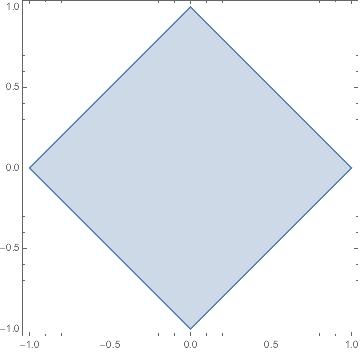
\includegraphics[width=.8\linewidth]{./norm-1.jpeg}
  \caption*{p = 1}
\end{subfigure}%
\begin{subfigure}{.33\textwidth}
  \centering
  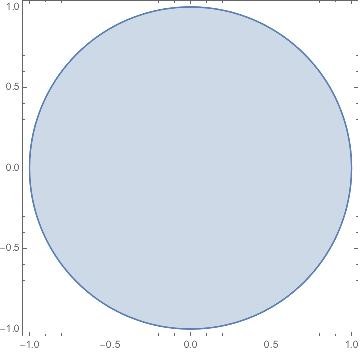
\includegraphics[width=.8\linewidth]{./norm-2.jpeg}
  \caption*{p = 2}
\end{subfigure}
\begin{subfigure}{.33\textwidth}
  \centering
  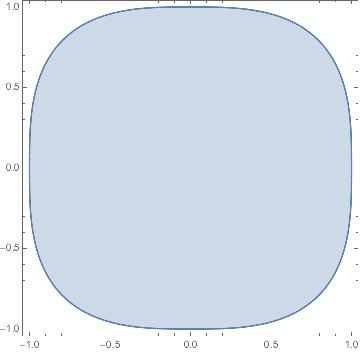
\includegraphics[width=.8\linewidth]{./norm-3.jpeg}
  \caption*{p = 3}
\end{subfigure}
\end{figure}

\begin{figure}[h]
\centering
\begin{subfigure}{.33\textwidth}
  \centering
  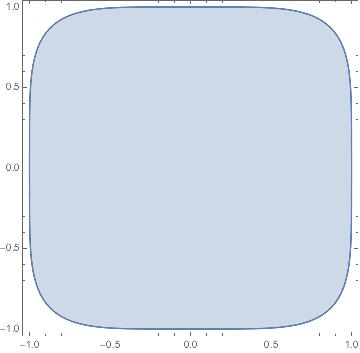
\includegraphics[width=.8\linewidth]{./norm-5.jpeg}
  \caption*{p = 5}
\end{subfigure}%
\begin{subfigure}{.33\textwidth}
  \centering
  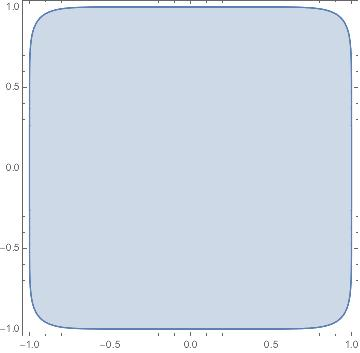
\includegraphics[width=.8\linewidth]{./norm-10.jpeg}
  \caption*{p = 10}
\end{subfigure}
\begin{subfigure}{.33\textwidth}
  \centering
  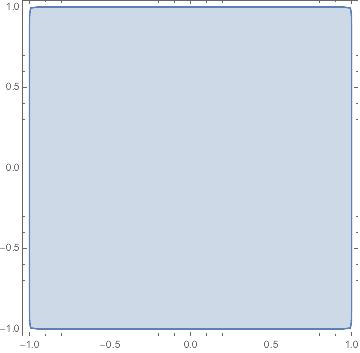
\includegraphics[width=.8\linewidth]{./norm-100.jpeg}
  \caption*{p = 100}
\end{subfigure}
\end{figure}
\newpage
\item Provide a proof that $$\max |x_i-y_i|=\lim_{p\rightarrow \infty}\left(\sum_{i=1}^n |x_i-y_i|^p\right)^{1/p}.$$

\begin{flushleft}
If the maximum value of $|x_i - y_i|$ occurs when $i = k$, let us set $\max |x_i - y_i| = |x_k - y_k|$.
$$ |x_k-y_k|^p \leq \sum_{i=1}^n |x_i-y_i|^p \leq n \cdot |x_k-y_k|^p $$

$$ \lim_{p\to\infty}\left(|x_k-y_k|^p\right)^{1/p} \leq \lim_{p\to\infty}\left(\sum_{i=1}^n |x_i-y_i|^p\right)^{1/p} \leq \lim_{p\to\infty}\left(n \cdot |x_k-y_k|^p\right)^{1/p}$$

$$ |x_k-y_k| \leq \lim_{p\to\infty}\left(\sum_{i=1}^n |x_i-y_i|^p\right)^{1/p} \leq \lim_{p\to\infty}(n^{1/p}) \cdot |x_k-y_k| = |x_k-y_k|$$
Using the squeeze theorem for sequences, since the sum is bounded on both sides by $|x_k-y_k|$, we have proven that the limit is equal to $|x_k-y_k| = \max |x_i - y_i|$. Therefore,

$$\max |x_i-y_i|=\lim_{p\rightarrow \infty}\left(\sum_{i=1}^n |x_i-y_i|^p\right)^{1/p} \Box$$

\end{flushleft}

\end{enumerate}
\item (2 points) Find an isometry (see Definition 2 on p.44) between $C_\infty[a,b]$ and $C_\infty[c,d]$ for any $a<b$ and $c<d$.

\begin{flushleft}
We need to find $T(x)$ such that:
$$ d_\infty(f,g) = \max_{x\in [a,b]} |f(x) - g(x)| = \max_{x\in [c,d]} |T(f(x)) - T(g(x))| = d_\infty(T(f),T(g)) $$
Let $T$ be the map between $C_\infty[c,d]$ and $C_\infty[a,b]$ defined as follows:
$$ (T\circ f)(x) = f\left(\frac{b-a}{d-c} (x-c) + a \right) $$
Since $x \in [c,d]$ if and only if $\frac{b-a}{d-c} (x-c) + a \in [a,b]$, we can say that $T\circ f$ is well-defined over $[c,d]$ and is a composition of well-defined functions. $T(ef + g) = eT(f) + T(g)$, so $T$ is a linear map.
$$ \| T\circ f\|_\infty = \max_{x\in [c,d]} |(T\circ f)(x)| = \max_{x\in [c,d]}\left|f\left(\frac{b-a}{d-c} (x-c) + a \right)\right| =  \left|f\left(\frac{b-a}{d-c} (y-c) + a \right)\right| = \max_{x\in [a,b]} |f(x)| = \| f\|_\infty $$

This equation is true for some $y \in [c,d]$ as $T\circ f$ is onto and $y$ corresponds to the maximum value
$$ d_\infty(f,g) = \|f-g\|_\infty = \|T(f-g)\| = \|T(f) - T(g)\| = d_\infty(T(f),T(g)) $$
$$ \Rightarrow d_\infty(f,g) = d_\infty(T(f),T(g)) \Leftrightarrow T \text{ is an isometry between } C_\infty[a,b] \text{ and } C_\infty[c,d] \, \Box$$.

\end{flushleft}
\end{enumerate}
\end{document}